\documentclass[a4paper]{article}
\usepackage[utf8]{inputenc}
\usepackage[russian,english]{babel}
\usepackage[T2A]{fontenc}
\usepackage[left=10mm, top=20mm, right=18mm, bottom=15mm, footskip=10mm]{geometry}
\usepackage{indentfirst}
\usepackage{amsmath,amssymb}
\usepackage[italicdiff]{physics}
\usepackage{graphicx}
\graphicspath{{images/}}
\DeclareGraphicsExtensions{.pdf,.png,.jpg}
\usepackage{wrapfig}

\usepackage{caption}
\captionsetup[figure]{name=Рисунок}
\captionsetup[table]{name=Таблица}

\title{\underline{Вопрос по выбору (Механика)}}
\author{Воронин Денис, Б04-403}
\date{}
\begin{document}

\maketitle
\begin{center}
\textbf{Обтекание тел, движущихся в газ (Эффект Магнуса)}
\end{center}

\section{Теоретические сведения}

Рассмотрим случай обтекания симметричного тела в газе.

\begin{wrapfigure}{l}{0.5\textwidth}
    \centering
    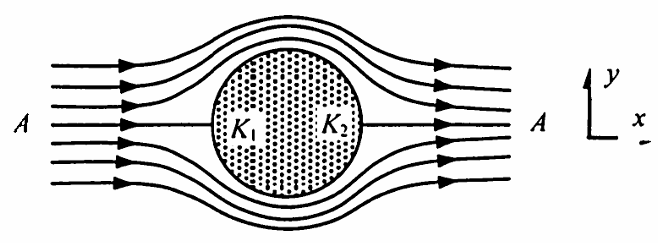
\includegraphics[width=0.4\textwidth]{pick1.PNG}
    \caption{Симметричное 
    тело в набегающем потоке воздуха}
\end{wrapfigure}

В этом случае воздух свободно (без трения) скользит по поверхности. На поверхности шара есть две точки ($K_{1}$ и $K_{2}$), в которых скорость 
течения обращается в нуль. Эти точки называются критическими. 
Согласно уравнению Бернулли:

\[P+ \frac{\rho \vartheta^{2}}{2} = const\] 

давление вдоль трубки тока не зависит от знака скорости. Поэтому распределения давлений перед телом и позади него одинаковы. Давления в 
критических точках, где скорость течения равна нулю ($\vartheta_{1}= \vartheta_{2} = 0$), совпадают и превышают давление вдали от тела.
Поскольку мы имеем дело с симметричным телом, то профиль давлений симметричен относительно оси АА. В итоге заключаем, что результирующая сил давления равна нулю. Это значит, что отсутствует сила сопротивления потоку, как нет и подъёмной силы:

\[F_{x} = F_{y} = 0\]

Этот результат связан с отсутствием вязкости: нет потерь энергии и импульса. Поэтому при равномерном обтекании тел 
любой формы сила сопротивления и подъёмная сила равны нулю.\par

\section{Экспериментальная часть}

Перейдем непосредственно к физическому явлению, которое присходит в эксперименте. 
Рассмотрим случай ,когда симметричное тело (цилиндр) движется в потоке воздуха, при этом имея угловую скорость вращения.


\begin{figure}[h]
\begin{center}
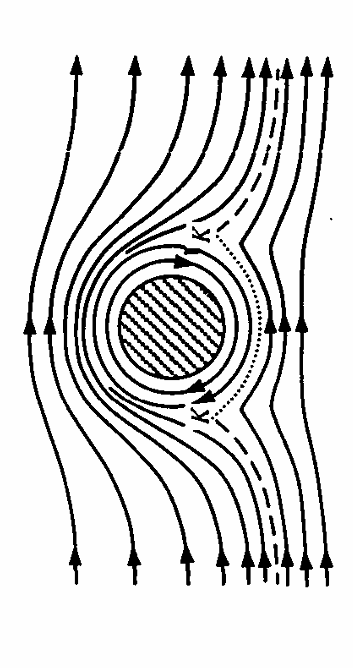
\includegraphics[width=0.20\textwidth]{pick2.PNG}
\caption{Свободное падение вращающегося цилиндра}
\end{center}
\end{figure}


\newpage

При свободном падении тела, на цилиндр набегают потоки воздуха, причем их концентрация слева и справа отличается.\par

Пусть вдали от тела скорость потока воздуха равна U. Вследствие 
вязкости скорость течения относительно поверхности тела обращается в 
нуль в точках поверхности и возрастает до значения $\sim U$ в пограничном 
слое . Если тело вращается, то его поверхность увлекает воздух. В результате возникает наложение двух течений:\par

1. Ламинарного обтекания и\par
2. циркуляции вокруг тела (вихревого обтекания)\par

Соответственно характерная скорость потока оказывается больше там, где 
линейная скорость точек тела направлена по скорости потока (на 
рисунке выше скорость потока слева от тела больше, чем справа).\par

Возрастание скорости течения справа от тела можно пояснить другим 
способом. За счёт увлечения потока вращающимся телом линии тока 
сгущаются слева, а справа разреживаются, в результате чего сечение трубок тока слева от тела уменьшается, и скорость потока в них возрастает 
согласно уравнению непрерывности pvS = const. Из уравнения Бернулли
$\frac{P}{\rho } + \frac{\vartheta^2}{2} = const  $ следует, что давление в некоторой области потока 
слева от тела оказывается меньше, чем справа: $P_{1}<P_{2}$, что и означает 
возникновение смещающей силы $F_{y}$.\par

\begin{wrapfigure}{r}{0.5\textwidth}
    \centering
    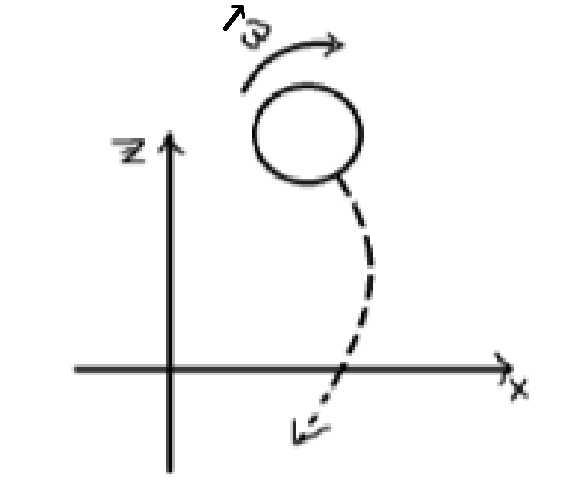
\includegraphics[width=0.25\textwidth]{pick3.PNG}
    \caption{Траектория цилиндра}
\end{wrapfigure}

Значение силы даётся формулой Жуковского-Кутта:
\[F_{y}^{(1)} = \text{Г}\rho U ,\text{Г} = \oint vdl \]

где U — скорость набегающего потока, $\rho  $ — плотность жидкости, а Г — 
циркуляция скорости вокруг тела. Это сила, приходящаяся на единицу 
длины тела, поперечной потоку. В частности, если тело есть цилиндр 
длиной l, то $F_{y} = lF_{y}^{(1)}$.

Пусть параметры цилиндра следующие: радиус - R, длина - l, угловая скорость - $\omega $, скорость набегающего потока - $\vartheta $.
Так как вблизи цилиндра $\vartheta_{R} = \omega R$, то $\text{Г} = 2\pi R \vartheta _{R} = 2\pi R^{2}\omega $\par

В итоге получаем: 
\[F = 2\pi \rho R^{2}\omega l\vartheta \]

Так как сила Магнуса направлена перпендикулярно скорости потока и перпендикулярно вектору угловой скорости,
то конечную формулу можно представить в виде:
\[F = 2\pi \rho R^{2}l\omega \times v\]

Пусть угловая скорость не меняется по мере падения цилиндра. Найдем уравнения, описывающие движение цилиндра:

\[mv' = mg + 2\pi \rho R^2l\omega \times v\]

Используя систему координат из рисунка выше имеем:
\[F_{x} = -2\pi \rho R^2l\omega \upsilon_{z}\]
\[F_{z} = 2\pi \rho R^2l\omega \upsilon_{x}\]

Соответственно уравнения движения цилиндра  принимают вид:
\[\upsilon'_{x} =- \varOmega\upsilon_{z}\]
\[\upsilon'_{z} =\varOmega\upsilon_{x} - g\] 
где $\varOmega = (2\pi \rho R^2l/m)\omega $. Если начальные условия $v_{x}(0) = 0 , v_{z}(0) = 0$ то 
\[\vartheta_{x} = \frac{g}{\varOmega }(1-cos\varOmega t) , \vartheta _{z} =-\frac{g}{\varOmega }sin\varOmega t\]  

Интерируя находим траекторию 
\[x = \frac{g}{\varOmega^2 }(\varOmega t-sin\varOmega t)\]
\[z =H - \frac{g}{\varOmega^2 }(1-cos\varOmega t)\]\par
\newpage

\begin{figure}[h]
\begin{center}
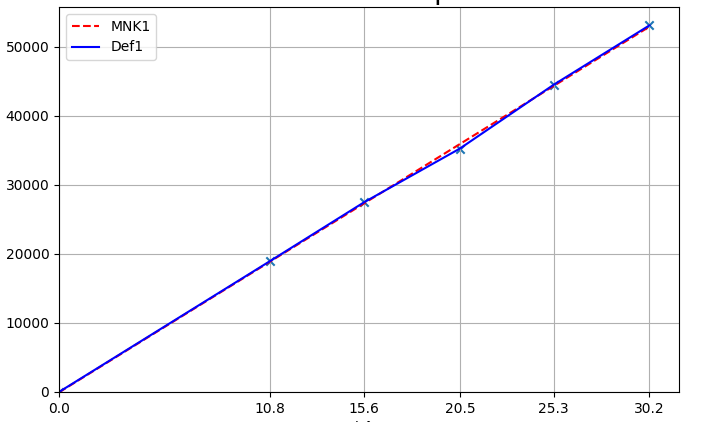
\includegraphics[width=0.9\textwidth]{pick4.PNG}
\caption{Зависимость силы, действующей на цилиндр от времени}
\end{center}
\end{figure}

\begin{figure}[h]
\begin{center}
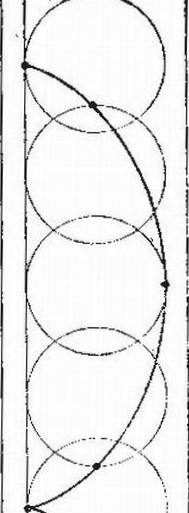
\includegraphics[width=0.145\textwidth]{pick5.jpg}
\caption{Траектория движения цилиндра}
\end{center}
\end{figure}

\end{document}